\documentclass[10pt]{article}
\usepackage[polish]{babel}
\usepackage[utf8]{inputenc}
\usepackage[T1]{fontenc}
\usepackage{amsmath}
\usepackage{amsfonts}
\usepackage{amssymb}
\usepackage[version=4]{mhchem}
\usepackage{stmaryrd}
\usepackage{graphicx}
\usepackage[export]{adjustbox}
\graphicspath{ {./images/} }

\title{Zadania - etap III (szkoła podstawowa) }

\author{}
\date{}


\begin{document}
\maketitle
CENTRUM NAUCZANIA MATEMATYKI\\
I KSZTALCENIA NA ODLEGłOŚĆ

Zadanie 1. Jaka jest ostatnia cyfra liczby: \(\left(5^{14}+10^{19}+9^{11}\right) \cdot\left(2^{53}+3^{21}\right) ?\)

Zadanie 2. Za każde bezbłędnie rozwiązane zadanie uczeń otrzymywał 10 punktów, a tracił 5 punktów za każde żle rozwiązane zadanie. Po rozwiązaniu 20 zadań uczeń otrzymał 80 punktów. Ile zadań uczeń rozwiązał dobrze a ile źle?

Zadanie 3. Podaj 183 cyfrę po przecinku w rozwinięciu dziesiętnym liczby \(\frac{7}{13}\).\\
Zadanie 4. Pole prostokąta \(\mathrm{ABCDprzedstawionego} \mathrm{na} \mathrm{poniższym} \mathrm{rysunku} \mathrm{wynosi} 42 \mathrm{~cm}^{2}\). Na boku ABwybrano punkt K różny od punktów A i B, a na boku CDwybrano punkt L różny od punktów Ci D. Wiemy, że pole trójkąta LDA jest równe \(7 \mathrm{~cm}^{2}\). Wykaż, że trójkąt CLK ma pole dwa razy większe od pola trójkąta LDA.\\
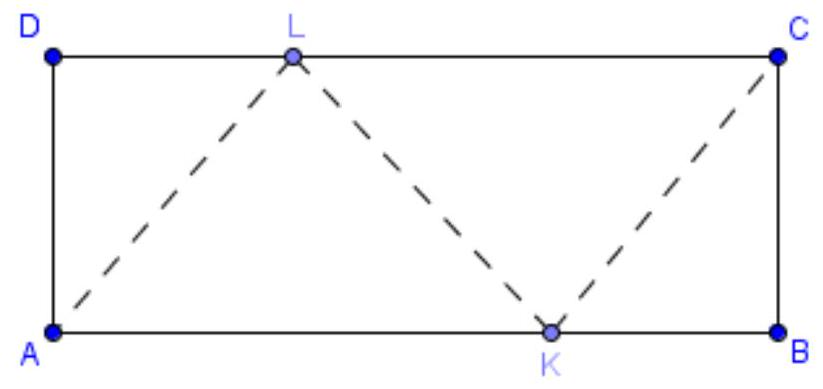
\includegraphics[max width=\textwidth, center]{2024_11_21_0222b9f9dea886a5ae2eg-1}

Zadanie 5. Dany jest kwadrat ABCDo polu równym \(36 \mathrm{~cm}^{2}\). Na bokach tego kwadratu zaznaczono środki boków, tak jak na poniższym rysunku. Ponadto punkt P jest środkiem odcinka KL.lle wynosi suma pól zakreskowanych czworokątów?\\
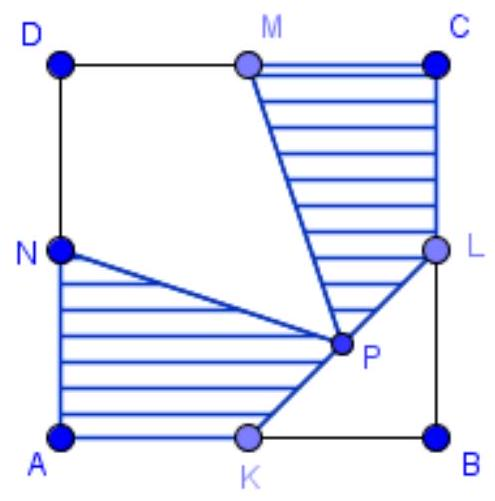
\includegraphics[max width=\textwidth, center]{2024_11_21_0222b9f9dea886a5ae2eg-1(1)}


\end{document}